\documentclass[a4paper,12pt]{article}

\usepackage{mystyle}

\usepackage{gensymb}
\usepackage{scalerel}
\usepackage{stackengine}

% \usepackage{skull}  % skull
\usepackage{halloweenmath}  % \bigpumpkin, skull (https://tug.ctan.org/info/symbols/comprehensive/symbols-a4.pdf -- Table 76)

\usepackage{tikzsymbols}

% https://tex.stackexchange.com/questions/3266/how-do-i-use-a-circle-as-a-math-accent-larger-than-mathring
% https://tex.stackexchange.com/a/3270/135045
\usepackage{accents}

\renewcommand{\mathring}[1]{\accentset{\circ}{#1}}


\graphicspath{ {images/} }


% https://tex.stackexchange.com/questions/5461/is-it-possible-to-change-the-size-of-an-arrowhead-in-tikz-pgf
\usetikzlibrary{arrows.meta}


\DeclareMathOperator{\Image}{Im}

\definecolor{pink}{RGB}{218, 3, 174}
\definecolor{violet}{RGB}{148, 0, 211}
\definecolor{green}{RGB}{0, 153, 0}
\definecolor{orange}{RGB}{255, 153, 0}
\definecolor{blue}{RGB}{5, 73, 255}
\definecolor{cyan}{RGB}{31, 206, 203}
\definecolor{cyan2}{RGB}{0, 166, 147}
\definecolor{cyangreen}{RGB}{0, 155, 118}
\definecolor{cyangreen2}{RGB}{0, 109, 91}


% https://tex.stackexchange.com/a/101138/135045

\newcommand\widesim[1]{\ThisStyle{%
  \setbox0=\hbox{$\SavedStyle#1$}%
  \stackengine{-.1\LMpt}{$\SavedStyle#1$}{%
    \stretchto{\scaleto{\SavedStyle\mkern.2mu\sim}{.5150\wd0}}{.6\ht0}%
  }{O}{c}{F}{T}{S}%
}}


\newcommand{\BigMiddleThree}{\;\left|\vphantom{\begin{pmatrix} 0\\0\\0 \end{pmatrix}}\right.\;}
\newcommand{\BigMiddleFour}{\;\left|\vphantom{\begin{pmatrix} 0\\0\\0\\0 \end{pmatrix}}\right.\;}


% https://tex.stackexchange.com/questions/63531/how-to-write-quotation-marks-in-math-environment
\DeclareMathSymbol{\mlq}{\mathord}{operators}{``}
\DeclareMathSymbol{\mrq}{\mathord}{operators}{`'}

% TODO: didn't work...
% \renewcommand{\Re}{\mathop{\mathrm{Re}}\nolimits}
% \renewcommand{\Im}{\mathop{\mathrm{Im}}\nolimits}

\DeclareMathOperator{\Arg}{Arg}
\DeclareMathOperator{\Real}{Re}
\DeclareMathOperator{\Imag}{Im}


% https://tex.stackexchange.com/questions/544453/undefined-control-sequence-after-paragraph
\renewcommand{\paragraph}[1]{\noindent\textbf{#1}\quad}


% https://tex.stackexchange.com/questions/36851/skipping-line-after-proof-in-proof-environment#comment73553_36851
\newcommand{\proofindent}{\hspace*{\fill}\par\vspace{0.5em}\noindent}


% https://tex.stackexchange.com/questions/4813/extendible-equals-sign
\makeatletter
\newcommand*{\Relbarfill@}{\arrowfill@\Relbar\Relbar\Relbar}
\newcommand*{\xeq}[2][]{\ext@arrow 0055\Relbarfill@{#1}{#2}}
\makeatother


% https://tex.stackexchange.com/questions/279100/typeset-the-shrug-%C2%AF-%E3%83%84-%C2%AF-emoji
\newcommand{\shrug}[1][]{%
\begin{tikzpicture}[baseline,x=0.8\ht\strutbox,y=0.8\ht\strutbox,line width=0.125ex,#1]
  \def\arm{(-2.5,0.95) to (-2,0.95) (-1.9,1) to (-1.5,0) (-1.35,0) to (-0.8,0)};
  \draw \arm;
  \draw[xscale=-1] \arm;
  \def\headpart{(0.6,0) arc[start angle=-40, end angle=40,x radius=0.6,y radius=0.8]};
  \draw \headpart;
  \draw[xscale=-1] \headpart;
  \def\eye{(-0.075,0.15) .. controls (0.02,0) .. (0.075,-0.15)};
  \draw[shift={(-0.3,0.8)}] \eye;
  \draw[shift={(0,0.85)}] \eye;
  % draw mouth
  \draw (-0.1,0.2) to [out=15,in=-100] (0.4,0.95); 
\end{tikzpicture}}



% https://tex.stackexchange.com/a/314638/135045
% \newcommand{\diff}{\mathop{}\!d\!}
\newcommand{\diff}{\mathop{}\!d}


% https://tex.stackexchange.com/questions/387570/how-to-make-cdot-operator-same-width-as-division-slash-operator-and-vice-ve
\newcommand*{\slashdiv}{\makebox[\widthof{${}\cdot{}$}]{{}/{}}}


\author{Алексеев Василий}


\title{Семинар 1}
\date{7 февраля 2025}


\begin{document}
  \maketitle
  
  \tableofcontents

  \thispagestyle{empty}
  
  \newpage
  
  
  
  \vspace*{\fill}
  
  \noindent
  \emph{
    К формулировкам и доказательствам (если такие вообще приводятся) стоит относиться критически.
    Основное в этом конспекте~---~решение задач (но ``критичность'' и здесь лучше не отключать).
    За строгой, ясной и последовательной теорией лучше обращаться к ``нормальным'' источникам.
    (Например, к лекциям.)
  }
  
  \vspace*{\fill}
  
  \thispagestyle{empty}
  
  \newpage
  
  
  \pagenumbering{arabic}


  \section{Числа (продолжение)}

  \subsection{Комплексные числа}
  
  %\begin{figure}[ht]
    %\centering
    %
\includegraphics[width=0.6\linewidth]{images/Apples}
    %
    %\caption{
      %Одно яблоко, два яблока, ...~---~натуральные числа используются при счёте предметов.
    %}
    %\label{fig:naturals}
  %\end{figure}
  
  
  % TODO:
  % [ ] Про комплексные:
  %   [ ] картинка с расширением чисел
  %   [X] определение,
  %   [X] операции + примеры,
  %   [ ] картинка с векторами,
  %   [X] тригонометрическая запись,
  %   [X] смысл за умножением + примеры + i^2,
  %   [X] показательная запись
  %   [X] про сравнение комплексных
  % [ ] Про интегралы
  %   [ ] определение
  %   [ ] табличные + вывод пары штук
  %   [ ] примеры (на рациональные и иррациональные)

  О компл\'{е}ксных числах можно думать как о расширении (ещё одном) понятия ``числа''~(\ref{fig:numbers-and-beyond}).

  \begin{figure}[ht]
    \centering
    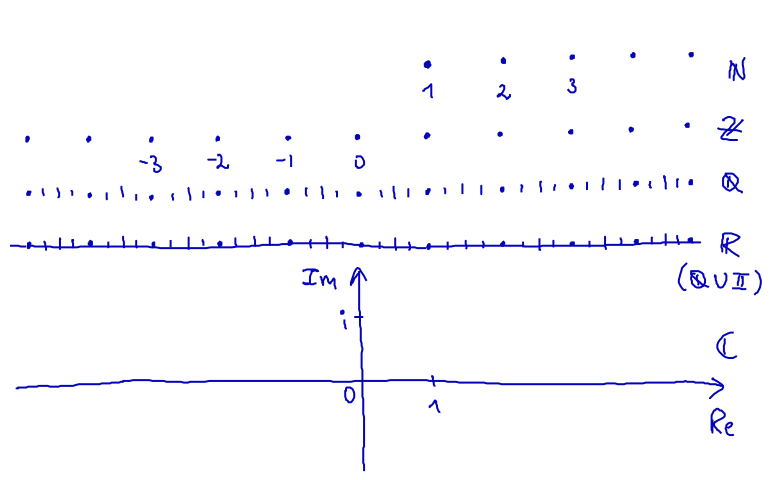
\includegraphics[width=0.8\linewidth]{images/numbers-and-beyond}
    
    \caption{
      ``Эволюция'' чисел.
      \emph{Натуральные}~---~использующиеся при счёте предметов (одно яблоко, два яблока, и так далее).
      Останемся справа от нуля и посмотрим, какие ещё есть числа.
      \emph{Рациональные}~---~доли от натуральных, ``деления на линейке'' ($1/2$, $3/4$ и так далее).
      \emph{Иррациональные}~---~``все оставшиеся'' (какие бы они ни были), не вошедшие в рациональные.
      Рациональные и иррациональные таким образом занимают весь луч от нуля до $+\infty$.
      Далее можно ввести \emph{отрицательные} числа: натуральные, ноль и противоположные натуральным объединяются в \emph{целые} числа.
      Рациональные и иррациональные просто ``расширяются'', включая теперь и отрицательные числа.
      Таким образом, занятой числами оказывается вся числовая прямая (числовая ось)~---~числа на ней называются \emph{действительными} числами.
      Но ведь можно, наверно, провести ещё одну ось?
      Тогда с числовой прямой выйдем на числовую плоскость~---~плоскость \emph{компл\'{е}ксных} чисел...
    }
    \label{fig:numbers-and-beyond}
  \end{figure}

  Комплексное число $z \hm\in \CC$ характеризуется двумя компонентами $(a, b)$, каждая из которых есть действительное число ($a, b \in \RR$) и показывает координату $z$ по оси: первая компонента $a$~---~по оси ``обычных'' действительных чисел (\emph{действительная часть} комплексного числа), вторая компонента~$b$~---~по новой оси, которая для работы с ``обычными'' числами не привлекалась (\emph{мнимая часть} комплексного числа).
  Записать комплексное число~$z$ можно так:
  \[
    z = a + i b
  \]
  где $i$~---~это так называемая \emph{мнимая единица} (единица, но не действительная, на новой оси).

  Для комплексных чисел естественным образом работают операции умножения на действительное число и сложения~(\ref{fig:alpha-mul-and-plus-for-c}): операции проводятся ``параллельно'' для каждой из компонент:
  \[
    \alpha z = \alpha (a + ib) = (\alpha a) + i (\alpha b),\quad \alpha \in \RR
  \]
  \[
    z_1 + z_2 = (a_1 + ib_1) + (a_2 + ib_2) = (a_1 + a_2) + i (b_1 + b_2)
  \]

  \begin{figure}[ht]
    \centering
    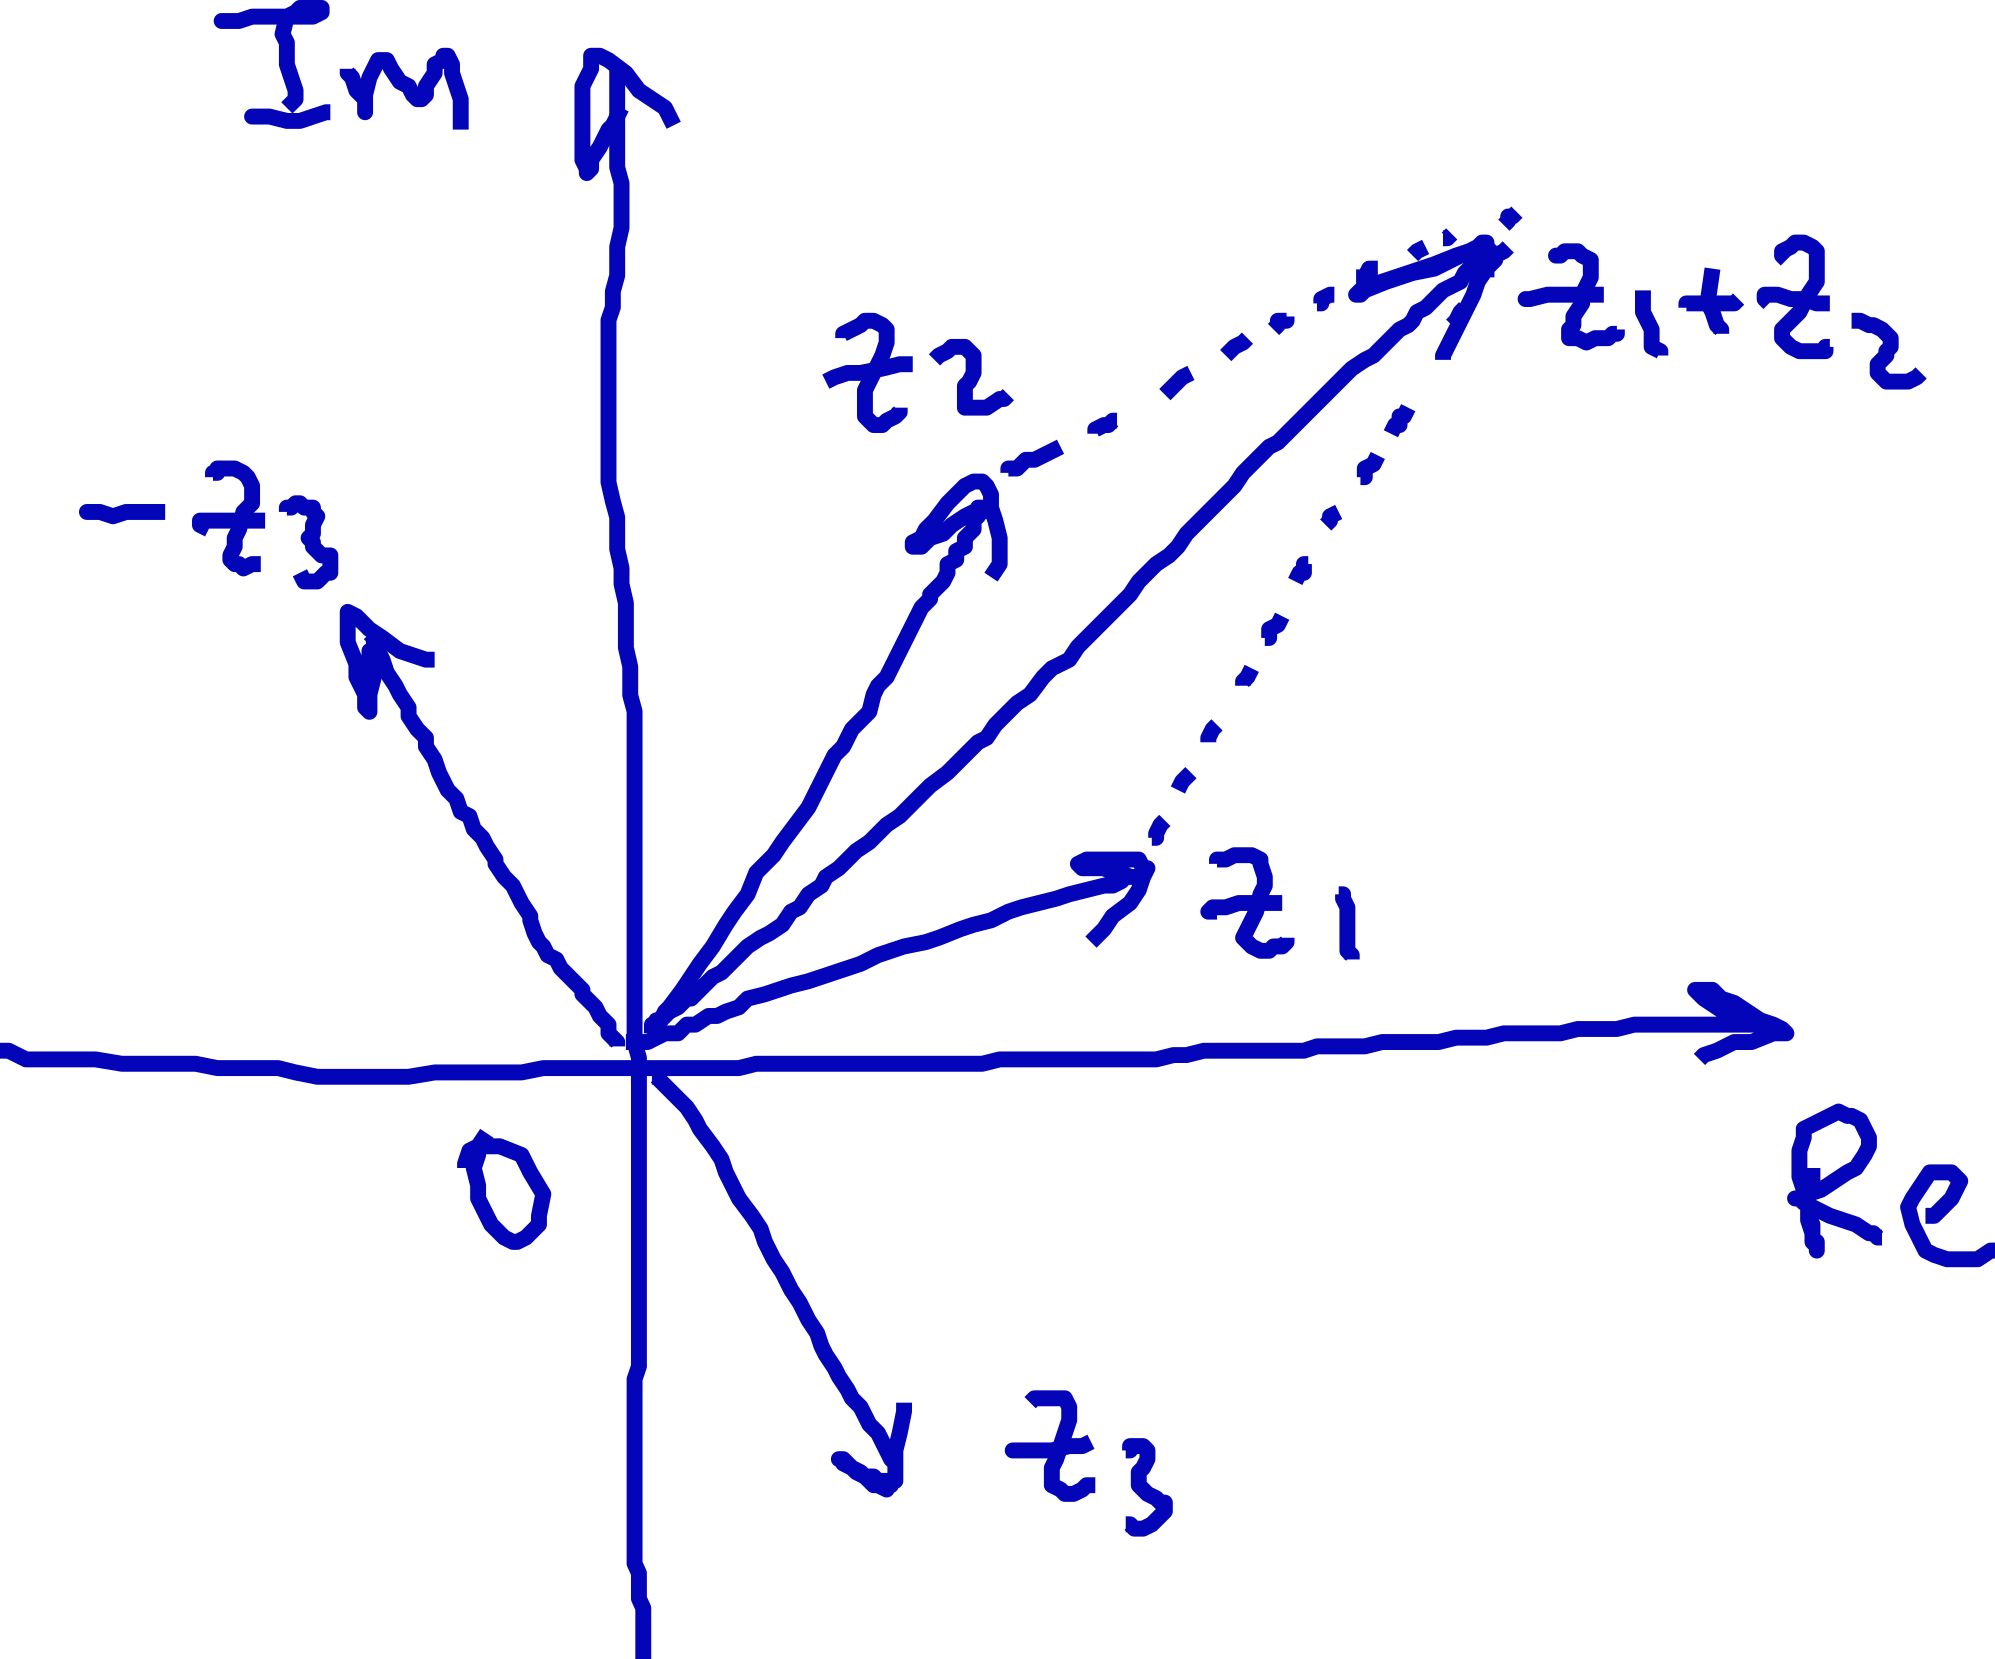
\includegraphics[width=0.6\linewidth]{images/alpha-mul-and-plus-for-c}
    
    \caption{
      При умножении комплексного числа на действительное число и сложении комплексных чисел происходят аналогичные операции с их радиус-векторами.
    }
    \label{fig:alpha-mul-and-plus-for-c}
  \end{figure}

  Но можно ли умножать и делить комплексные числа?
  Да, но эти операции расширяются на комплексные числа уже не так очевидно.\footnote{
    По крайней мере, по мнению составляющего конспект.
  }
  Поэтому введём их, а потом ещё раз вернёмся к ним чуть позже (в попытке осознать).
  При умножении работают обычные правила раскрытия скобок и раздельного сложения компонент разной природы далее.
  Однако при умножении друг на друга собственно комплексных чисел (``чисел с $i$''), включается ещё одно правило:
  \begin{equation}\label{eq:im-i}
      i^2 = -1
  \end{equation}
  (Таким образом, ``мнимость'' $i$ открывается с новой стороны: теперь это не просто ``другая'' единица (по новой оси, которой раньше не было), а такое число, которое в квадрате даёт $1$ (таких чисел тоже раньше не было).)

  \begin{example}
    Перемножим два числа: $z_1 \hm= a_1 \hm+ i b_1$ и $z_2 \hm= a_2 \hm+ i b_2$.
    \[
      z_1 \cdot z_2 = (a_1 \hm+ i b_1) \cdot (a_2 \hm+ i b_2) = \blacktriangle
    \]
    Будем раскрывать скобки, сразу собирая вместе все составляющие действительной и мнимой частей числа-результата (и имея в виду правило~\eqref{eq:im-i}):
    \[
      \blacktriangle = (a_1 a_2 - b_1 b_2) + i(a_1 b_2 + a_2 b_1)
    \]
  \end{example}

  Деление~---~действие из той же ``плоскости'', что и умножение.
  Поэтому посмотрим ещё пример на деление.

  \begin{example}
    Поделим друг на друга два числа: $z_1 \hm= a_1 \hm+ i b_1$ и $z_2 \hm= a_2 \hm+ i b_2$ ($z_2 \hm{\not=} 0$).
    \[
      \frac{z_1}{z_2} = \frac{a_1 \hm+ i b_1}{a_2 \hm+ i b_2} = \blacktriangle
    \]
    Что значит: ``поделить'' два комплексных числа?
    Можем считать, что это значит~---~найти результат деления, представив его в форме, использующейся для записи комплексных чисел.
    Для этого надо каким-то образом избавиться от комплексности в знаменателе.
    Пользуются следующим ``трюком'': домножим числитель и знаменатель на $a_2 \hm- i b_2$ (то есть на число, отличающееся от знаменателя знаком мнимой части):
    \[
      \blacktriangle = \frac{(a_1 a_2 + b_1 b_2) + i(-a_1 b_2 + a_2 b_1)}{a_2^2 + b_2^2}
    \]
    Далее дробь уже можно разложить в сумму двух: с~$i$ и без~$i$.

    Для числа, отличающегося от данного~$z \hm= a \hm+ ib$ знаком мнимой части, вводят специальное название: \emph{комплексно сопряжённое} числу $z$ число.
    И обозначают как $\overline{z}$.
    Таким образом, $\overline{z} \hm= a \hm- ib$.
    % TODO: \bar didn't work for some reason...
  \end{example}

  \medskip
  
  Познакомимся с ещё одним способом записи комплексного числа~---~\emph{тригонометрическим}.
  
  Суть этого способа в том, чтобы расписать радиус-вектор~$\bds r$ комплексного числа как сумму проекций: на действительную и на мнимую оси~(\ref{fig:z-projection}):
  \begin{equation}\label{eq:trig-z}
    z = 1 \cdot r\cos \phi + i \cdot r \sin \phi = r(\cos \phi + i \sin \phi)
  \end{equation}
  где $r \hm= |\bds r|$ есть длина соответствующего~$z$ радиуса-вектора, а $\phi$~---~это угол между радиусом-вектором и положительным направлением оси~$\Real$ (больший нуля, если отсчитывается против часовой стрелки, иначе меньше нуля).
  (Для $z \hm= 0$ длина радиуса-вектора равна нулю, а угол~$\phi$ не определён.)

  Число $r$ называется также \emph{модулем} комплексного числа~$z$, и может обозначаться как~$|z|$.
  Угол же~$\phi$, очевидно, определён не однозначно, а с точностью до $2\pi$ (от одного или нескольких дополнительных поворотов на $2\pi$ против или по часовой стрелке ничего по сути не поменяется).  % TODO: check language
  Всё множество таких углов $\phi$, могущих участвовать в формуле~\eqref{eq:trig-z} и отличающихся на сколько-то $2 \pi$, называется аргументом комплексного числа:
  \[
    \Arg(z) = \{\phi + 2\pi k \mid k \in \ZZ\}
  \]

  Для определённости, из всего этого множества углов можно выделить один~---~лежащий в полуинтервале~$(-\pi, \pi]$.
  Такое значение аргумента числа~$z$ обозначается как~$\arg(z)$.

  \begin{figure}[ht]
    \centering
    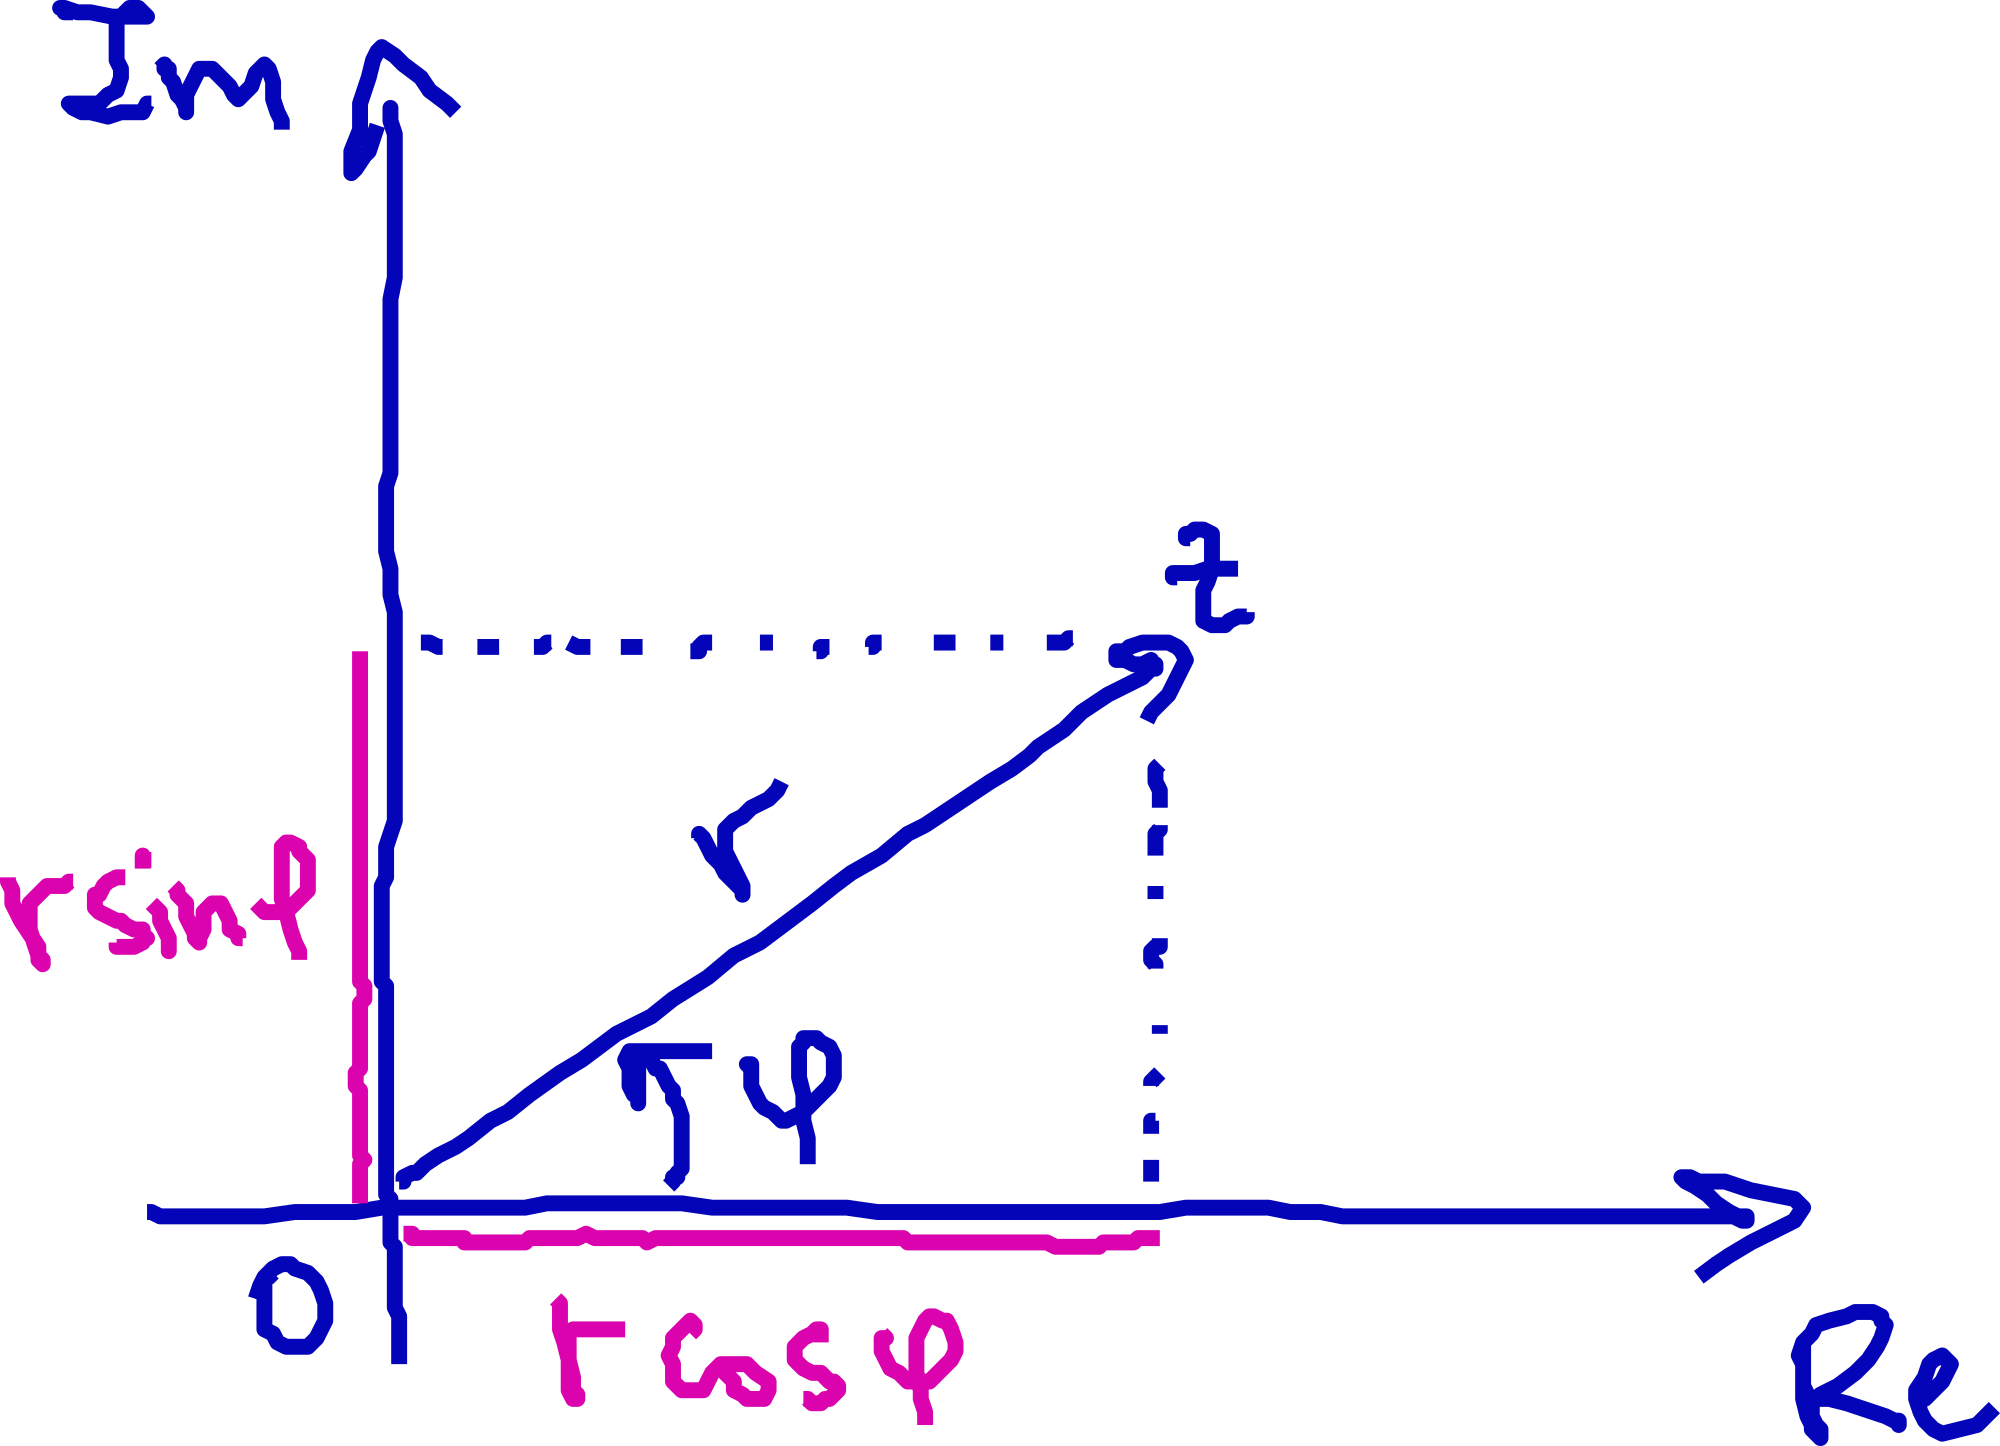
\includegraphics[width=0.6\linewidth]{images/z-projection}
    
    \caption{
      % TODO: ввести Re и Im как обозначения
      Если радиус-вектор комплексного числа по длине равен~$r$ и образует угол~$\phi$ с положительным направлением оси~$\Real$, то его проекции на оси~$\Real$ и~$\Imag$ будут соответственно равны $r \cos \phi$ и $r \sin \phi$.
    }
    \label{fig:z-projection}
  \end{figure}

  Вернёмся к умножению комплексных чисел, но посмотрим на него с числами в тригонометрической записи:
  \begin{equation}\label{eq:c-mul}
    \begin{aligned}
      &z_1 = r_1(\cos \phi_1 + i \sin\phi_1),\quad z_2 = r_2(\cos \phi_2 + i \sin\phi_2)\\
      &z_1 \cdot z_2 = \ldots = r_1 r_2 \bigl(\cos (\phi_1 + \phi_2) + i\sin (\phi_1 + \phi_2)\bigr)
    \end{aligned}
  \end{equation}
  То есть длина радиуса-вектора результата~---~произведение длин векторов умножаемых чисел, а угол~---~сумма углов.

  Деление:
  \[
    \begin{aligned}
      &z_1 = r_1(\cos \phi_1 + i \sin\phi_1),\quad z_2 = r_2(\cos \phi_2 + i \sin\phi_2)\\
      &\frac{z_1}{z_2} = \ldots = \frac{r_1}{r_2} \bigl(\cos (\phi_1 - \phi_2) + i\sin (\phi_1 - \phi_2)\bigr)
    \end{aligned}
  \]
  То есть модуль частного~---~частное модулей, а угол~---~разность углов.

  Более очевидна связь между делением и умножением.
  И понятен ``физический смысл'' таким образом введённой операции умножения.

  \begin{example}
    Во-первых, умножение действительных чисел укладывается в такую общую (более сложную) схему.
    Например, $1 \cdot 2 \hm= 2$: модули перемножились, а угол $0 \hm= 0 \hm+ 0$~---~остался нулевым.

    Далее, свойство мнимой единицы: $i^2 \hm= -1$.
    Модуль остался единичным.
    Угол стал равным: $\frac{\pi}{2} \hm+ \frac{\pi}{2} \hm= \pi$~---~то есть радиус-вектор мнимой единицы при возведении её в квадрат поворачивается против часовой стрелки ещё на $\frac{\pi}{2}$.
    И число в результате оказывается уже на другой оси~---~на оси действительных чисел, причём в отрицательной половине~(\ref{fig:i-i}).

    \begin{figure}[ht]
      \centering
      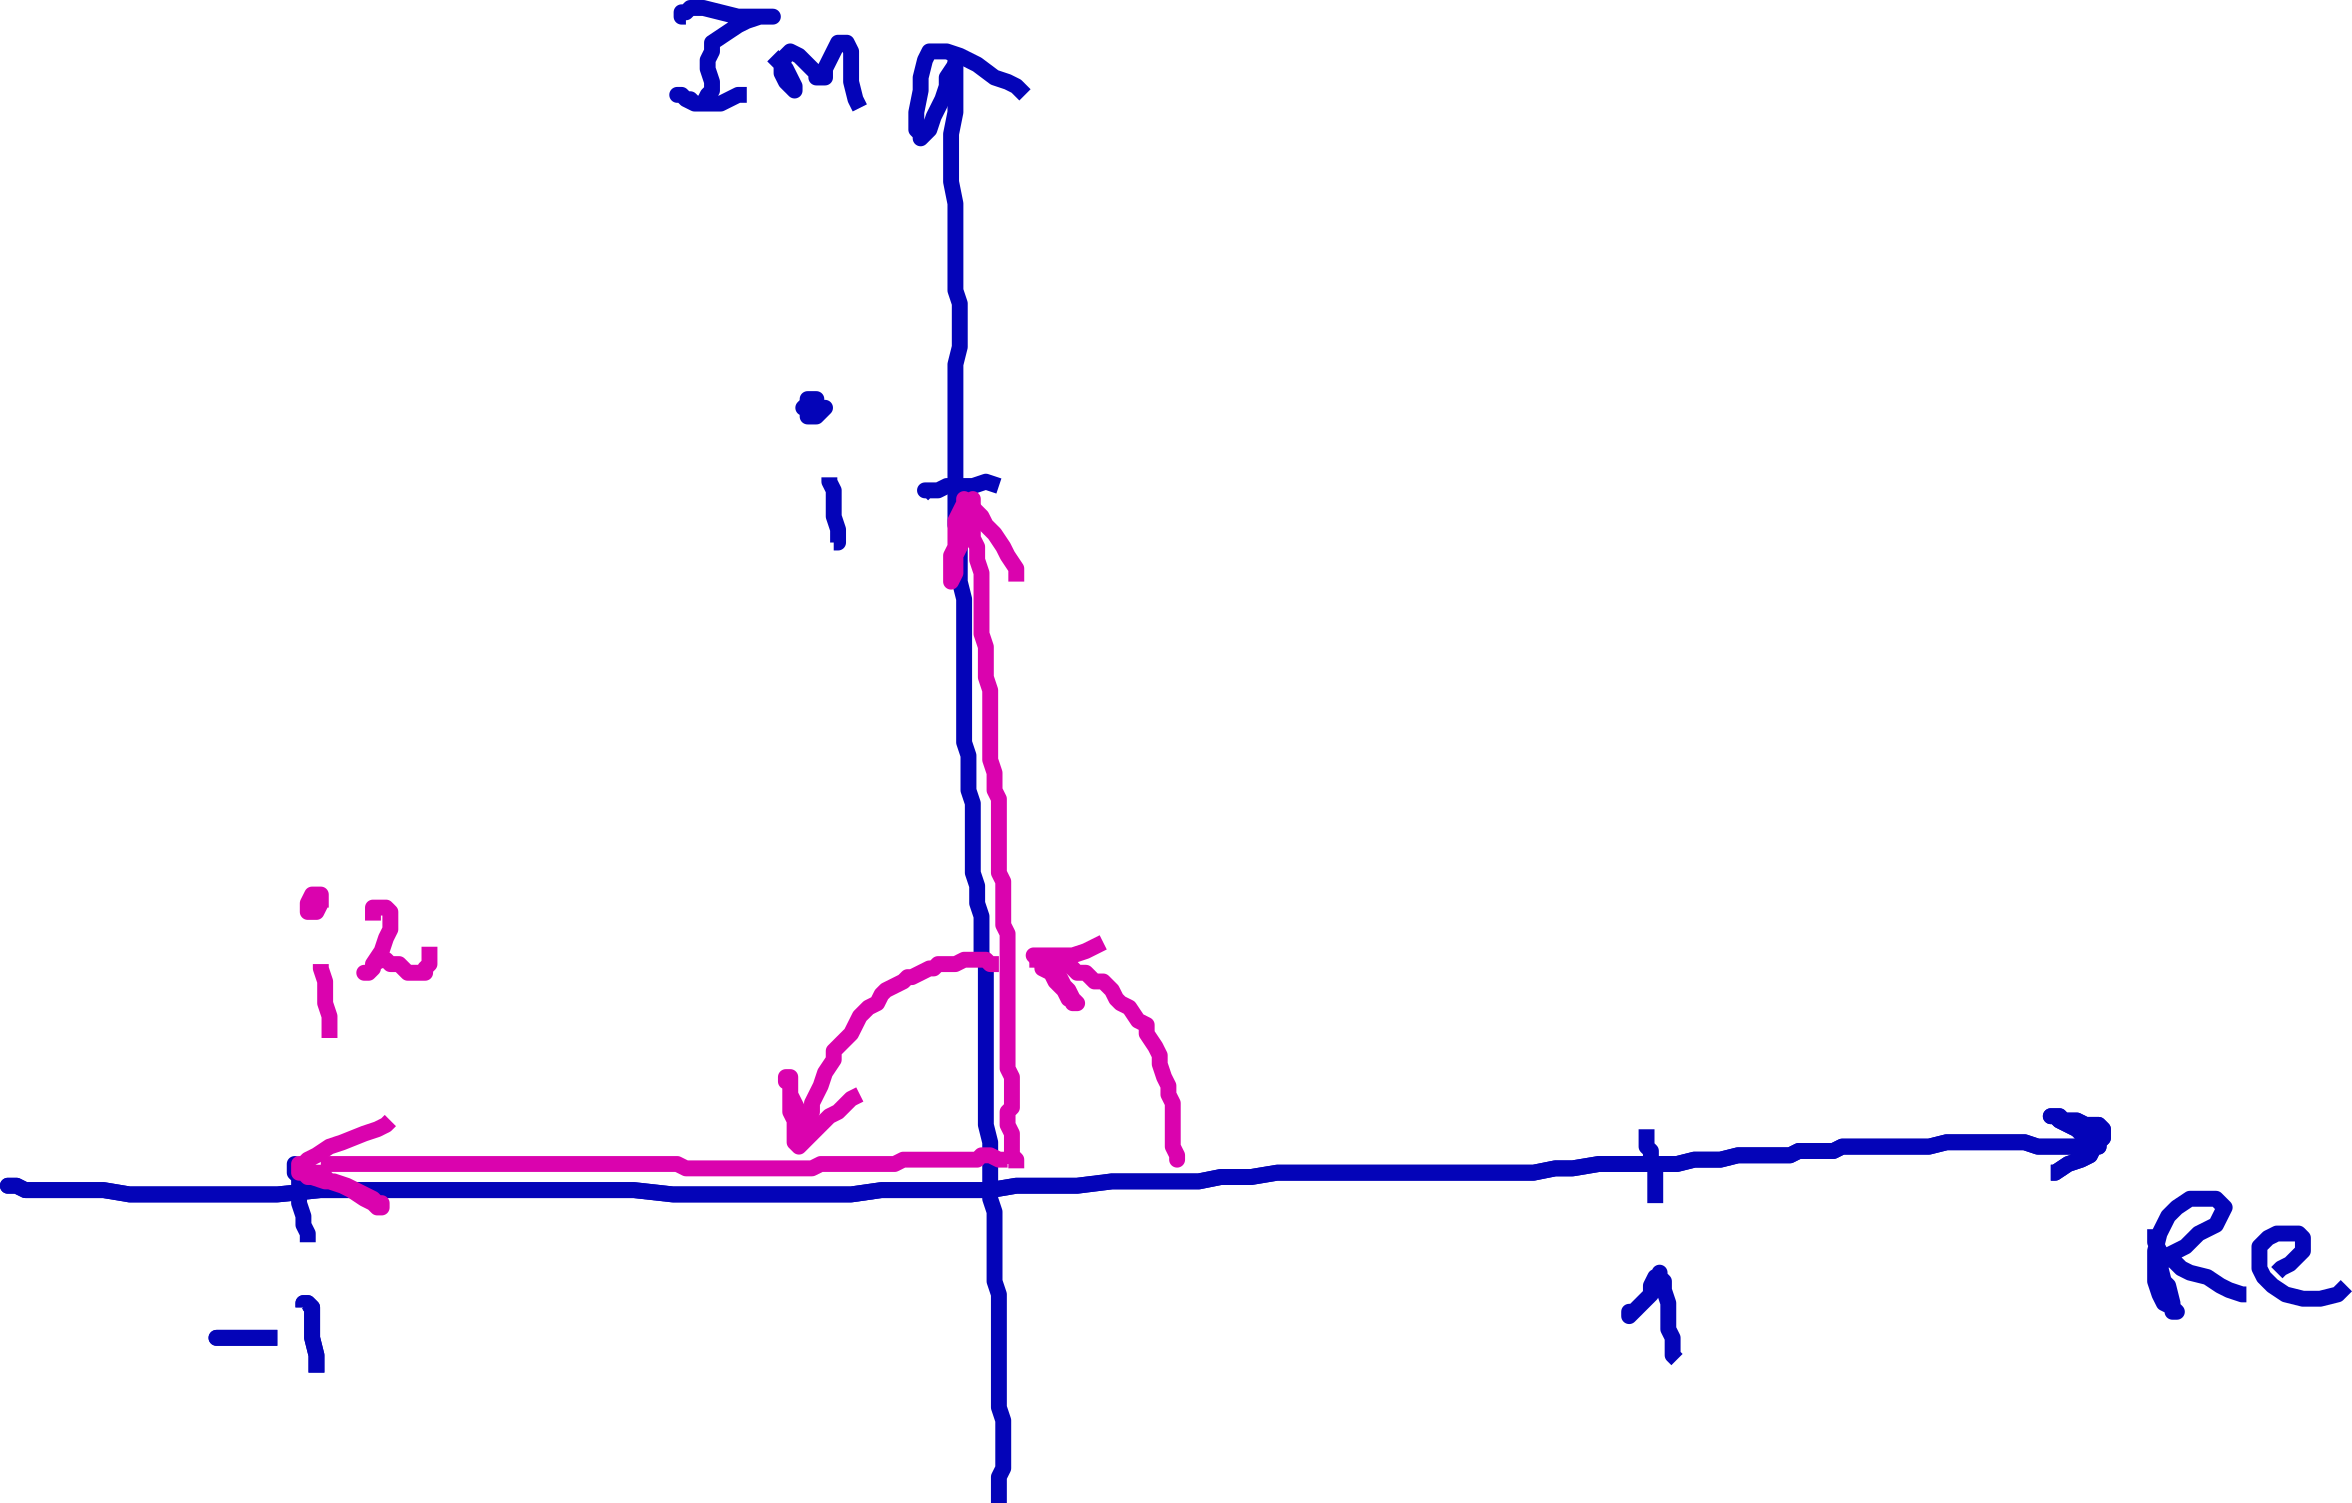
\includegraphics[width=0.6\linewidth]{images/i-i}
    
      \caption{
        Радиус-вектор числа~$i^2$.
      }
      \label{fig:i-i}
    \end{figure}
  \end{example}

  Имея в виду логику операций умножения и деления комплексных чисел (если смотреть на них в тригонометрической записи), можно прийти к ещё одному способу записи комплексных чисел~---~\emph{показательному}:
  \begin{equation}
      z \hm= r(\cos \phi + i \sin \phi) \Leftrightarrow \boxed{
          z = re^{i\phi}
      }
  \end{equation}

  В таком виде умножение и деление будут проходить так:
  \[
    \begin{aligned}
      &z_1 \cdot z_2 = r_1e^{i\phi_1} \cdot r_2e^{i\phi_2} = r_1 r_2 e^{i(\phi_1 + \phi_2)}\\
      &z_1 \slashdiv z_2 = r_1e^{i\phi_1} \slashdiv r_2e^{i\phi_2} = \frac{r_1}{r_2} e^{i(\phi_1 - \phi_2)}
    \end{aligned}
  \]

  Поэтому на показательную запись комплексного числа можно смотреть просто как на ``компактную и более удобную тригонометрическую'' (преобразования модулей и углов такие же, просто более очевидные), а не буквально как на ``е в степени''.
  % TODO: заметка про возможность буквального прочтения

  \medskip

  Отдельно отметим в конце невозможность сравнения комплексных чисел через ``больше/меньше''.
  Потому что, например, для действительных чисел выражение $x \hm< y$ говорило о том, левее ли лежит число~$x$ на числовой прямой, чем число~$y$.
  Но как читать запись ``$z_1 \hm< z_2$'', ведь на плоскости нет ``левее'' и ``правее''?
  Поэтому про сравнение комплексных ``не говорят'', сравнивать их можно либо на равенство (``равно/не равно''), либо по модулям: запись $|z_1| \hm< |z_2|$ имеет смысл.\footnote{
    Сравнение комплексных по модулю по сути говорит о том, какое из них находится дальше от начала координат.
    При сравнении действительных тоже учитывается дальность от нуля, но кроме неё~---~ещё и то, с какой стороны от нуля расположено число.
  }


  \subsubsection{Новый взгляд на квадратное уравнение с отрицательным дискриминантом}

  Решим уравнение:
  \begin{equation}\label{eq:cubic-for-quadratic}
    z^3 = 1
  \end{equation}

  Очевидный корень: $z \hm= 1$.
  Есть ли ещё?
  (Очевидный ответ: нет.)
  Подойдём к вопросу основательнее: соберём всё в левой части и разложим на множители:
  \[
    z^3 - 1 = 0
  \]
  \[
    (z - 1)(z^2 + z + 1) = 0
  \]

  Такое уравнение равносильно совокупности:
  \[
    \left[
      \begin{aligned}
          &z - 1 = 0\\
          &z^2 + z + 1 = 0
      \end{aligned}
    \right.
  \]

  Рассмотрим отдельно получившееся квадратное уравнение.
  Его дискриминант:
  \[
    D = 1^2 - 4 = -3 < 0
  \]

  Корней нет?
  Нет, но только действительных.
  Комплексные же корни есть:
  \[ % TODO: pink
    z_{1, 2} = \frac{-1 \pm \sqrt{\textcolor{pink}{-}3}}{2} = \frac{-1 \pm \sqrt{3\textcolor{pink}{i^2}}}{2} = \frac{-1 \pm i\sqrt{3}}{2}
  \]
  % TODO: отметить про вершины правильного многоугольника в номере про уравнение далее

  Итого, получаем три корня:
  \[
    \left[
      \begin{aligned}
          &z = 0\\
          &z = \frac{-1 \pm i\sqrt{3}}{2}
      \end{aligned}
    \right.
  \]

  Отметим интереса ради корни на комплексной плоскости.
  Для этого определим ещё модуль и аргумент комплексных корней:
  \[
    z = \frac{-1 \pm i\sqrt{3}}{2} = 1 \cdot \left(-\frac{1}{2} \pm i\frac{\sqrt{3}}{2}\right)
    % = r(\cos\phi + i\sin\phi),\quad \left\{
    %   \begin{aligned}
    %     &r = 1\\
    %     &\phi = 2\pi/3\ \mbox{или}\ \phi = 4\pi/3
    %   \end{aligned}
    % \right.
  \]

  Таким образом, $r \hm= 1$ и $\phi \hm= 2\pi/3$ или $\phi \hm= 4\pi/3$.

  Получается, все три корня уравнения~\eqref{eq:cubic-for-quadratic} лежат на окружности радиуса единица и с центром в нуле, причём они также являются вершинами правильного треугольника (комплексные корни получаются из $z \hm= 1$, если поворачивать его радиус-вектор на угол $2\pi/3$ против часовой стрелки)~(\ref{fig:cubic-roots}).

  \begin{figure}[ht]
    \centering
    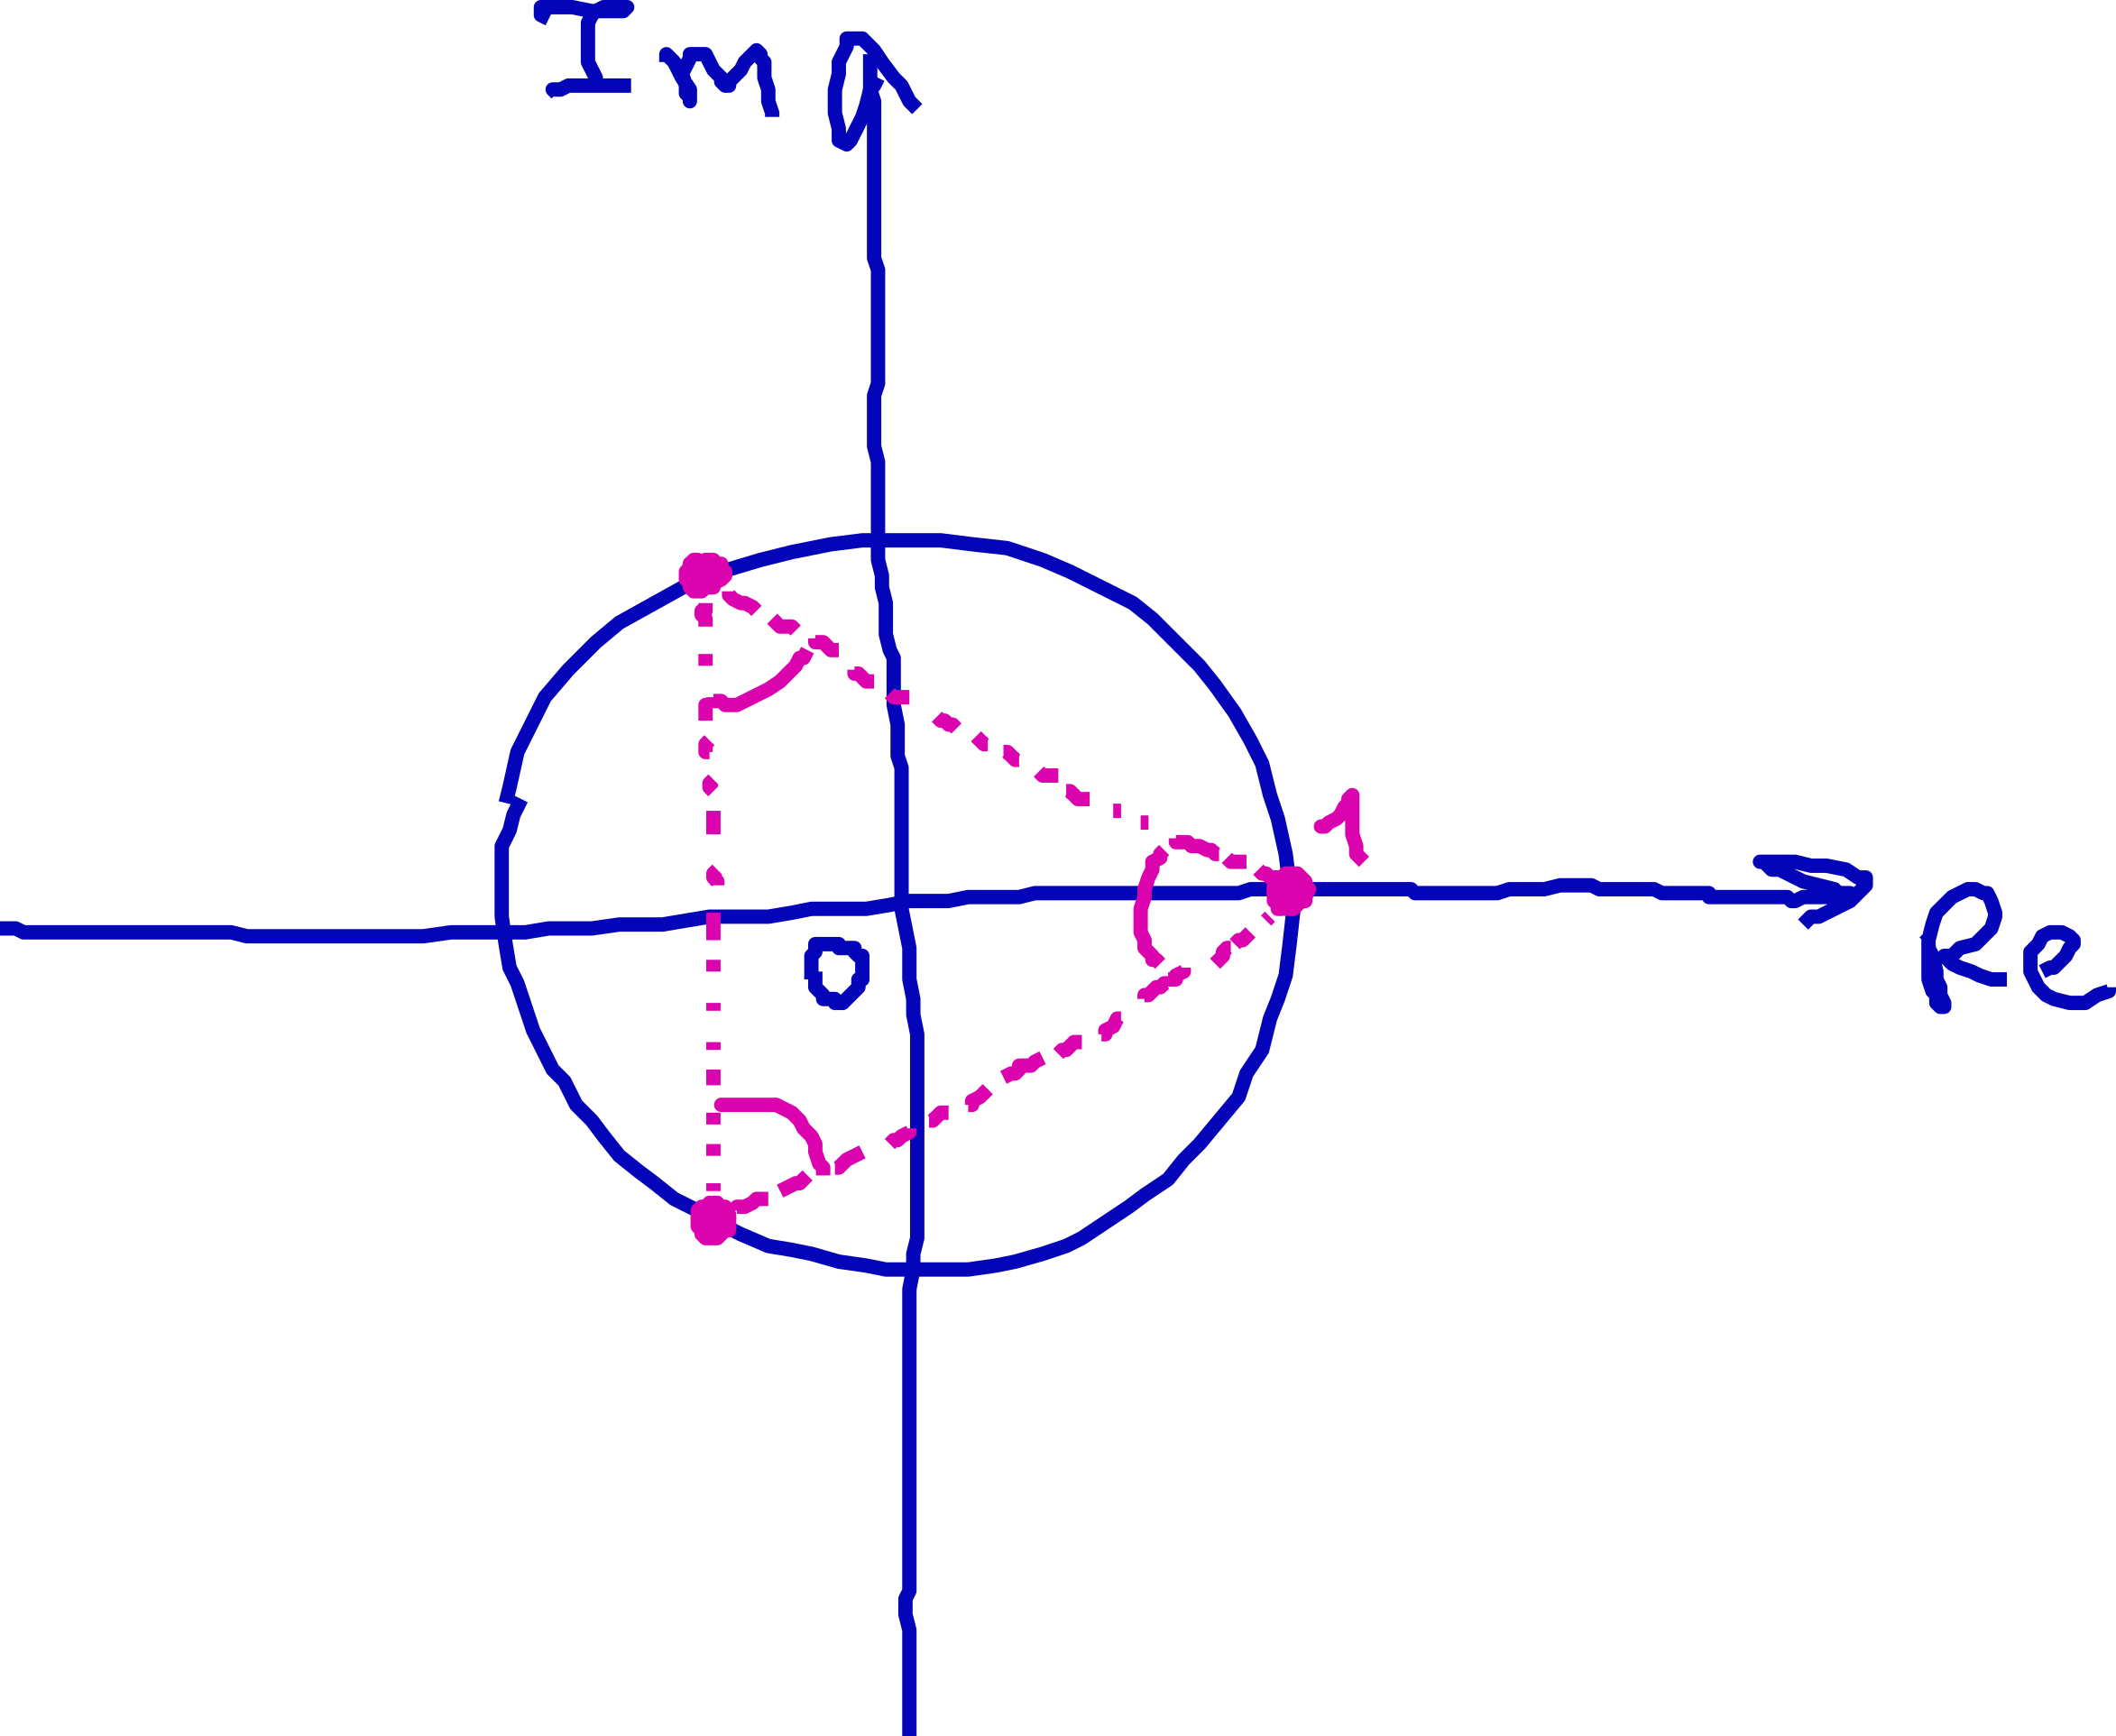
\includegraphics[width=0.6\linewidth]{images/cubic-roots}
    
    \caption{
      Корни уравнения~$z^3 = 1$ на комплексной плоскости.
    }
    \label{fig:cubic-roots}
  \end{figure}

  
  \subsubsection{С1, \S 5, \textnumero 15(3)}

  Найти множество точек комплексной плоскости, заданное условием:
  \[
    |z + 2i - 1| \leq 2
  \]
  
  \begin{solution}
    Немного перепишем неравенство:
    \[
      \bigl|z - (1 - 2i)\bigr| \leq 2
    \]

    Теперь видно, что неравенство определяет точки, удалённые от числа~$(1 \hm- 2i)$ на расстояние не более~$2$~(\ref{fig:z-zc}).
    А это~---~круг радиуса~$2$ с центром в указанной точке. % TODO: picture
    
    \begin{figure}[ht]
      \centering
      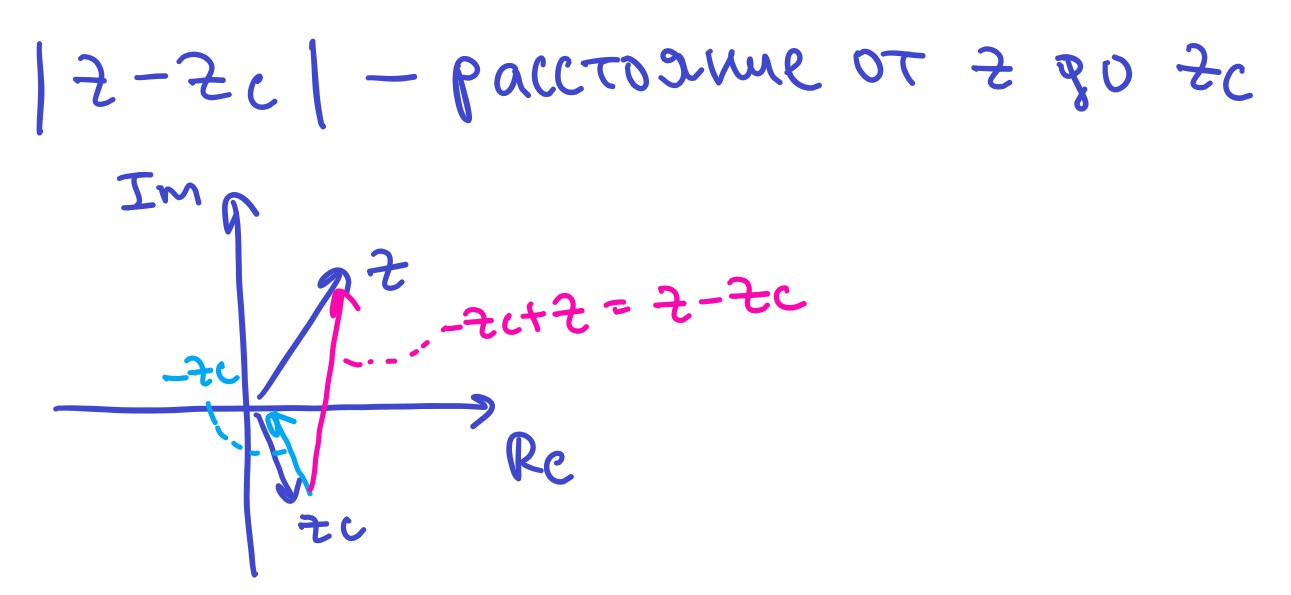
\includegraphics[width=0.8\linewidth]{images/z-zc}
    
      \caption{
        $z \hm- z_c$~---~вектор из числа $z_c$ в $z$, а его длина~$|z \hm- z_c|$~---~это расстояние между $z$ и $z_c$.
      }
      \label{fig:z-zc}
    \end{figure}
  \end{solution}


  \subsubsection{С1, \S 5, \textnumero 31(1)}

  Записать комплексное число в тригонометрической форме:
  \[
    z = \left(\sqrt{3} - i\right)^{100}
  \]

  % TODO: модуль комплексного числа: a^2 + b^2, z \bar z = |z|^2 (добавить выше)
  \begin{solution}
    (Возводить скобку в сотую степень ``в лоб'', очевидно, не вариант.)

    Начнём с того, что представим в тригонометрической форме число в скобке.
    (Далее возвести его в сотую степень будет несложно~\eqref{eq:c-mul}.)
    \[
      \sqrt{3} - i = 2 \left(\frac{\sqrt 3}{2} - \frac{i}{2}\right) = r (\cos\phi + i \sin\phi)
    \]
    где $r \hm\equiv 2$, а $\phi$~---~такой угол, что $\cos\phi \hm= \frac{\sqrt 3}{2}$ и $\sin\phi \hm= -\frac{1}{2}$; то есть $\phi$ можно взять равным $-\frac{\pi}{6}$.

    Возвращаясь в возведению в сотую степень:
    \[
      z = \bigl(r (\cos\phi + i \sin\phi)\bigr)^{100} = \left(r e^{i \phi}\right)^{100} = r^{100} (\cos{100 \phi} + i \sin{100 \phi})
    \]

    Число найдено.
    Остаётся привести ``адекватное'' значение аргумента. % TODO: проверить ответ для этого номера в конце задачника
    Найдём $\arg(z)$:
    \[
      100 \phi + 2 \pi k \in (-\pi, \pi] \Rightarrow k = \?
    \]
    \[
      100 \phi + 2 \pi k = 2 \pi k - \frac{100 \pi}{6} = \frac{12 \pi k - 100 \pi}{6}
    \]

    Получаем, что $k \hm= 8$, и $\arg(z) \hm= -\frac{2 \pi}{3}$.
  \end{solution}

  
  \subsubsection{С1, \S 5, \textnumero 32(4)}

  Найти все корни уравнения:
  \[
    z^8 = 1 + i
  \]
  
  \begin{solution}
    Будем искать $z$ в виде $z \hm= r (\cos\phi \hm+ i\sin\phi)$.
    Тогда $z^8 \hm= r^8 (\cos{8\phi} \hm+ i\sin{8\phi})$.
    Правую часть уравнения также представим в тригонометрической форме:
    \[
      1 + i = \sqrt{2} \left(\frac{1}{\sqrt{2}} + \frac{i}{\sqrt{2}}\right) = \sqrt{2} \left(\cos{\frac{\pi}{4}} + i \sin{\frac{\pi}{4}}\right)
    \]

    Уравнение:
    \[
      r^8 (\cos{8\phi} \hm+ i\sin{8\phi}) = \sqrt{2} \left(\cos{\frac{\pi}{4}} + i \sin{\frac{\pi}{4}}\right)
    \]

    равносильно следующей системе:
    \[
      \left\{
        \begin{aligned}
          &r^8 = \sqrt{2}\\
          &8\phi = \frac{\pi}{4} + 2\pi k,\ k \in \ZZ
        \end{aligned}
      \right.
    \]

    Рассмотрим отдельно выражение для определения аргумента:
    \[
      8\phi = \frac{\pi}{4} + 2\pi k \quad\Leftrightarrow \quad \phi = \frac{\pi + 8\pi k}{32}
    \]

    Видно, что при $k \hm= 8$ получим $\phi \hm= \frac{\pi}{32} \hm+ 2\pi$~---~то есть по сути то же самое, что и $\phi \hm= \frac{\pi}{32}$.
    Очевидно, в этот момент всё ``зацикливается'' и далее углы будут повторяться.
    Поэтому уникальные углы определяются $k \hm= 0,\, 1, \ldots, 7$.

    Итого, корни уравнения:  % TODO: picture?
    \[
      \left\{
        r (\cos\phi + i \sin \phi) \BigMiddleThree \:\begin{aligned}
          &r = 2^{1/16}\\
          &\phi = \frac{\pi + 8\pi k}{32},\ k = 0,\,1,\ldots, 7
        \end{aligned}
      \right\}
    \]
  \end{solution}



  \section{Неопределённый интеграл (продолжение)}
  
  Вспомним кое-что из интегралов.
  
  Первообразной функции~$f(x)$ на каком-то промежутке называется функция~$F(x)$, производная которой равна этой функции на данном промежутке:
  \[
    F'(x) = f(x)
  \]
  
  Неопределённым интегралом от функции~$f(x)$ называется совокупность первообразных этой функции:
  \[
    \int f(x) \diff x = \{F(x) + C \mid C \in \RR\} = F(x) + C
  \]

  Связь между производной функции и её дифференциалом:
  \[
    \diff f(x) = f'(x) \diff x
  \]

  Интеграл от суммы равен сумме интегралов, а числовой коэффициент можно выносить за знак интеграла:
  \[
    \begin{aligned}
      &\int\bigl(f(x) + g(x)\bigr) \diff x = \int f(x) \diff x + \int g(x) \diff x\\
      &\int \alpha f(x) \diff x = \alpha \int f(x) \diff x,\quad \alpha \in \RR
    \end{aligned}
  \]

  При интегрировании перед заменой переменной могут использоваться такие ``приёмы'' для получения нужного выражения под дифференциалом:
  \[
    \begin{aligned}
      &\diff x = \diff (x + C)\\
      &\diff x = \frac{1}{a} \diff (ax)
    \end{aligned}
  \]

  Вспомним некоторые ``табличные'' интегралы.

  \[
    \int x^{\alpha} \diff x = \frac{x^{\alpha + 1}}{\alpha + 1} + C,\quad \alpha \not= -1
  \]
  \[
    \int \frac{1}{x} \diff x = \ln |x| + C
  \]

  Интегралы от тригонометрических функций:
  \[
    \int \sin x \diff x = {-}\cos x + C  % TODO: excess space?
  \]
  \[
    \int \cos x \diff x = \sin x + C
  \]

  Интегралы от показательной функции:
  \[
    \int e^x \diff x = e^x + C
  \]

  \[
    \int a^x \diff x = \int e^{x \ln a} \diff x = \frac{1}{\ln a} \int e^{x \ln a} \diff(x \ln a) = \frac{a^x}{\ln a} + C
  \]

  Вместо аккуратного вывода последний интеграл можно было вывести и ``догадыванием'':
  \[
      F'(x) = a^x \Rightarrow F(x) = \? \quad \ldots \quad F(x) = \frac{a^x}{\ln a}
  \]

  Ещё интегралы от тригонометрических и обратных тригонометрических функций:
  \[
    \int \frac{1}{\cos^2 x} \diff x = \tg x + C
  \]
  \[
    \int \frac{1}{\sqrt{1 - x^2}} \diff x = \arcsin x + C
  \]

  Последний интеграл можно немного усложнить:
  \begin{equation}\label{eq:int-to-arcsin}
  \begin{split}
    \int \frac{1}{\sqrt{a^2 - x^2}} \diff x
      &= \frac{1}{a} \int \frac{1}{\sqrt{1 - \left(\frac{x}{a}\right)^2}} \diff x\\
      &= \int \frac{1}{\sqrt{1 - \left(\frac{x}{a}\right)^2}} \diff \left(\frac{x}{a}\right)
      = \arcsin\left(\frac{x}{a}\right) + C,\quad (a > 0)
  \end{split}
  \end{equation}
  
  Интеграл, сводящийся к арктангенсу:
  \[
    \int \frac{1}{1 + x^2} \diff x = \arctg x + C
  \]

  Снова можно аналогичным образом усложнить:\footnote{
    И можно заметить, что от знака~$a$ уже ничего зависеть не будет.
  }
  \begin{equation}
  \begin{split}\label{eq:int-to-arctg}
    \int \frac{1}{a^2 + x^2} \diff x
      &= \frac{1}{a^2} \int \frac{1}{1 + \left(\frac{x}{a}\right)^2} \diff x\\
      &= \frac{1}{a} \int \frac{1}{1 + \left(\frac{x}{a}\right)^2} \diff \left(\frac{x}{a}\right)
      = \frac{1}{a} \arctg\left(\frac{x}{a}\right) + C
  \end{split}
  \end{equation}

  Интегралы от гиперболических функций:
  \[
    \int \sh x \diff x = \ch x + C
  \]
  \[
    \int \ch x \diff x = \sh x + C
  \]
  \[
    \int \frac{1}{\ch^2 x} \diff x = \th x + C
  \]

  % TODO: обратные гиперболические функции?

  И ещё пара интегралов, которые можно получить небольшой ``модификацией'' подынтегральных функций в~\eqref{eq:int-to-arctg} и~\eqref{eq:int-to-arcsin}.

  ``Высокий логарифм'':
  \begin{equation}
  \begin{split}
    \int \frac{1}{x^2 - a^2} \diff x
      &= \int \frac{1}{(x - a)(x + a)} \diff x\\
      &= \frac{1}{2a} \int \left(\frac{1}{x - a} - \frac{1}{x + a}\right) \diff x\\
      &= \frac{1}{2a} \ln\left|\frac{x - a}{x + a}\right| + C
  \end{split}
  \end{equation}

  ``Длинный логарифм'':
  \begin{equation*}
  \begin{split}
    \int \frac{1}{\sqrt{x^2 - a^2}} \diff x
      &= \frac{1}{a} \int \frac{1}{\sqrt{\left(\frac{x}{a}\right)^2 - 1}} \diff x\\
      &= \int \frac{1}{\sqrt{\left(\frac{x}{a}\right)^2 - 1}} \diff\left(\frac{x}{a}\right) = \blacktriangle
  \end{split}
  \end{equation*}

  Можно сделать замену:\footnote{
    Для простоты считаем, что $x\hm/a \hm> 0$, то есть что $x$ и $a$ одинаковых знаков.
  }
  \[  % TODO: уточнить про знак икса? (больше нуля)
    % \begin{aligned}
      \frac{x}{a} \equiv \ch t,\quad t > 0\quad (\Rightarrow \sh t > 0)
    %   &x = a \ch t\\
    %   &\diff x = a \sh t \diff t
    % \end{aligned}
  \]
  \[
    \blacktriangle = \int \frac{1}{\sh t} \sh t \diff t = t + C = \spadesuit
  \]

  Теперь надо сделать обратную замену...
  \[
    \frac{x}{a} \equiv \ch t = \frac{e^t + e^{-t}}{2} \Rightarrow t = \?
  \]

  Пусть $e^t \hm\equiv z$ ($t \hm> 0 \hm\Rightarrow e^t \hm> 1$).
  Тогда $e^{-t} \hm= 1\hm/ z$ и приходим к уравнению:
  \[
    \begin{aligned}
      &\frac{x}{a} = \frac{z}{2} + \frac{1}{2z}\\
      &a \cdot z^2-2x \cdot z + a = 0
    \end{aligned}
  \]

  Корни которого:
  \[
    z_{1,2} = \frac{x \pm \sqrt{x^2 - a^2}}{a}
  \]

  Так как $z \hm= e^t$ и далее $x\hm/a \hm= (e^t \hm+ e^{-t}) \hm/ 2$, то понимаем, что один корень~$z$ будет соответствовать значению~$t \hm> 0$, а второй~---~значению~$t \hm< 0$.
  Раз хотим найти $t \hm> 0$, то, очевидно, оставляем~$z$ с ``плюсом'':
  \[
    z = \frac{x + \sqrt{x^2 - a^2}}{a}
  \]

  Тогда:
  \[
    \begin{aligned}
      &e^t = \frac{x + \sqrt{x^2 - a^2}}{a}\\
      &t = \ln \left(\frac{x + \sqrt{x^2 - a^2}}{a}\right)
    \end{aligned}
  \]

  И наконец можно довести до конца интеграл:\footnote{
    В конце ставим под интегралом модуль, потому что~$x$ вообще может быть и отрицательный.
  }
  \[
    \spadesuit = \ln \left(\frac{x + \sqrt{x^2 - a^2}}{a}\right) + C = \ln \left|x + \sqrt{x^2 - a^2}\right| + C
  \]

  Аналогично, можно бы было найти и такой интеграл, где бы под корнем была не разность квадратов, а сумма.
  Итого, обобщая, ``длинный логарифм'':
  \[
    \int \frac{1}{\sqrt{x^2 \pm a^2}} \diff x = \ln \left|x + \sqrt{x^2 \pm a^2}\right| + C
  \]
  

  \subsection{Интегралы от рациональных функций}
  
  \subsubsection{С2, \S 2, \textnumero 3(2)}

  Найти интеграл:
  \begin{equation}\label{eq:2-3(2)-int}
    \int \frac{x^2 + 2}{(x - 1) (x + 1)^2} \diff x
  \end{equation}
  
  \begin{solution}
    Общий метод нахождения подобных интегралов~---~разложение ``сложной'' подынтегральной дроби (правильной, у которой степень многочлена числителя меньше степени многочлена знаменателя) в сумму дробей ``попроще'' (тоже правильных), каждая из которых уже интегрируется (более-менее понятным способом).

    В знаменателе подынтегральной функции стоит произведение $(x \hm- 1) (x \hm+ 1)^2$.
    Какие знаменатели, таким образом, могли бы быть у дробей-слагаемых, суммой которых представима дробь под интегралом?
    Очевидно, знаменатели могли быть такими: $(x \hm- 1)$, $(x \hm+ 1)$, $(x \hm+ 1)^2$, $(x \hm- 1)(x \hm+ 1)$.
    Последний вариант $(x \hm- 1)(x \hm+ 1)$ можно ``отсечь'', потому дробь в таким знаменателем, в свою очередь, могла бы быть получена как сумма дробей со знаменателями $(x \hm- 1)$ и $(x \hm+ 1)$.
    Итого, надо искать три слагаемых, со знаменателями: $(x \hm- 1)$, $(x \hm+ 1)$, $(x \hm+ 1)^2$.

    Что можно сказать про числители?
    Так как слагаемые тоже должны быть правильными дробями,\footnote{
      Можно бы было допустить и неправильные дроби в слагаемых, но тогда коэффициенты напротив икс в ``неправильных'' степенях должны были бы занулиться. 
    } в общем виде можно записать такое разложение:
    \[
      \frac{x^2 + 2}{(x - 1) (x + 1)^2} = \frac{A}{x - 1} + \frac{B}{x + 1} + \frac{Cx + D}{(x + 1)^2}
    \]

    Вместо поиска слагаемого $\frac{Cx + D}{(x + 1)^2}$ можно искать слагаемое вида $\frac{C}{(x + 1)^2}$~---~это не ограничит возможности, потому что
    \[
      \frac{B}{x + 1} + \frac{C}{(x + 1)^2} = \frac{Bx + (B + C)}{(x + 1)^2}
    \]
    то есть любое слагаемое вида $\frac{Cx + D}{(x + 1)^2}$ можно получить как сумму дробей $\frac{B}{x + 1}$ и $\frac{C}{(x + 1)^2}$ с нужными коэффициентами.

    Поэтому будем искать разложение в виде:\footnote{
      Заметим, что из рассуждения выше вытекает, что можно бы было искать разложение и в таком виде:
      \[
        \frac{x^2 + 2}{(x - 1) (x + 1)^2} = \frac{A}{x - 1} + \frac{Bx + C}{(x + 1)^2}
      \]
      В любом случае видно, что степень многочлена в знаменателе раскладываемой в сумму дроби определяет количество ``степеней свободы''~---~сколько коэффициентов надо будет искать справа.
    }
    \begin{equation}\label{eq:2-3(2)-finding-fractions}
        \frac{x^2 + 2}{(x - 1) (x + 1)^2} = \frac{A}{x - 1} + \frac{B}{x + 1} + \frac{C}{(x + 1)^2}
    \end{equation}

    Приведём сумму справа к общему знаменателю (обратно):
    \[
      \frac{x^2 + 2}{(x - 1) (x + 1)^2} = \frac{A(x + 1)^2 + B(x + 1)(x - 1) + C(x - 1)}{(x - 1) (x + 1)^2}
    \]

    Это равенство равносильно следующему:
    \[
      x^2 + 2 = A(x + 1)^2 + B(x + 1)(x - 1) + C(x - 1),\quad x \not= \pm 1
    \]

    Два многочлена равны во всех точках, кроме, возможно, нескольких ($\RR \hm\setminus \{\pm 1\}$).
    (Или, иначе, если собрать всё в одной части и приравнять нулю~---~многочлен равен нулю во всех точках, кроме, возможно, нескольких.)
    Отсюда можно заключить, что равенство должно быть верным вообще при всех~$x$:
    \begin{equation}\label{eq:2-3(2)-finding-coeffs}
        x^2 + 2 = A(x + 1)^2 + B(x + 1)(x - 1) + C(x - 1)
    \end{equation}

    А значит, можно просто приравнять коэффициенты при~$x$ в одинаковых степенях слева и справа:
    \[
      \left\{
        \begin{aligned}
          &1 = A + B\\
          &0 = 2A + C\\
          &2 = A - B - C
        \end{aligned}
      \right.
    \]
    Система три на три, её можно решить (наверно%\footnote{
      %Точно, потому что строчки линейно независимы: если ко второй прибавить третью, коэффициент $C$ уйдёт, и останется только в третьей строке~---~таким образом, третью строчку нельзя будет представить как сумму первых двух.
    %}).  % TODO: make some explanation
    ).

    Но рассмотрим подробнее другой способ поиска коэффициентов в~\eqref{eq:2-3(2)-finding-coeffs}.
    Раз равенство должно быть верным при всех $x$, значит... можно просто взять и подставить в него какие-то ``удобные'' икс!
    \[
      \begin{aligned}
        &x = -1\colon\quad 1 + 2 = 0 + 0 - 2C \Rightarrow \boxed{C = -3/2}\\
        &x = \hphantom{-}1\colon\quad 1 + 2 = 4A + 0 + 0 \Rightarrow \boxed{A = 3/4}\\
        &x = \hphantom{-}0\colon\quad 0 + 2 = A - B - C \Rightarrow \boxed{B = 1/4}
      \end{aligned}
    \]

    Итак, разложение ``сложной'' подынтегральной дроби по ``простым''~\eqref{eq:2-3(2)-finding-fractions} найдено:
    \[
      \frac{x^2 + 2}{(x - 1) (x + 1)^2} = \frac{3/4}{x - 1} + \frac{1/4}{x + 1} + \frac{-3/2}{(x + 1)^2}
    \]

    И интеграл~\eqref{eq:2-3(2)-int} может быть найден как сумма интегралов:
    \[
      \int \frac{x^2 + 2}{(x - 1) (x + 1)^2} \diff x
        = \int \frac{3/4}{x - 1} \diff x
        + \int \frac{1/4}{x + 1} \diff x
        + \int \frac{-3/2}{(x + 1)^2} \diff x
    \]

    Первый ``простой'' интеграл:
    \[
      \int \frac{3/4}{x - 1} \diff x = \frac{3}{4} \int \frac{1}{x - 1} \diff(x - 1) = \frac{3}{4} \ln|x - 1| + C
    \]

    Второй (из той же серии):
    \[
      \int \frac{1/4}{x + 1} \diff x = \ldots = \frac{1}{4} \ln|x + 1| + C
    \]

    % TODO: Упс, перебор, это к следующему номеру
    % Чтобы взять третий, выделим в числителе производную знаменателя:\footnote{
    %   Чтобы прийти к интегралу вида:
    %   \[
    %     \int \frac{f'(x)}{f(x)} \diff x = \int \frac{1}{f(x)} \diff f(x) = \ln\bigl|f(x)\bigr| + C
    %   \]
    %   где в процессе использована связь между производной и дифференциалом функции:
    %   \[
    %     \diff f(x) = f'(x) \diff x
    %   \]
    % }
    % \[
    %   \left((x + 1)^2\right)' = 2x + 2
    % \]
    % \[
    %   \int \frac{-3/2}{(x + 1)^2} \diff x
    %   = -\frac{3}{2} \int \frac{1}{(x + 1)^2} \diff x
    %   \xrightarrow{\left((x + 1)^2\right)' = 2x + 2}
    % \]

    И третий:
    \[
      \int \frac{-3/2}{(x + 1)^2} \diff x = -\frac{3}{2} \int \frac{1}{(x + 1)^2} \diff (x + 1) = -\frac{3}{2} \frac{(x + 1)^{-2 + 1}}{-2 + 1} + C = \frac{3}{2(x + 1)} + C
    \]

    Итоговый интеграл:
    \[
      \frac{3}{4} \ln|x - 1| + \frac{1}{4} \ln|x + 1| + \frac{3}{2(x + 1)} + C
    \]
  \end{solution}


  \subsubsection{С2, \S 2, \textnumero 4(2)}

  Найти интеграл:
  \[
    \int \frac{1}{x^3 + 1} \diff x
  \]

  % TODO: пример с неправильной
  \begin{solution}
    Подынтегральная дробь правильная (выделять целую часть не надо).
    Поэтому разложим на множители знаменатель:
    \[
      x^3 + 1 = (x + 1)(x^2 - x + 1)
    \]

    % TODO: про комплексные
    Этот номер отличается от предыдущего тем, что теперь в разложении оказывается ``скобка'' с икс в квадрате, и с ней уже ничего сделать нельзя (так как дискриминант отрицательный (а мы ``забываем'' про комплексные и снова работаем с действительными числами)).\footnote{
      Но можно сделать и с комплексными корнями:
      \[
        x^2 - x + 1 = 0 \Rightarrow x_{1, 2} = \frac{1 \pm i \sqrt{3}}{2}
      \]

      Тогда разложение дроби в сумму можно искать точно по такой же схеме, как в номере ранее:  % TODO: ref
      \[
        \frac{1}{(x + 1)\bigl(x - (1/2 + i\sqrt{3}/2)\bigr)\bigl(x - (1/2 - i\sqrt{3}/2)\bigr)} = \frac{A}{x + 1} + \frac{B}{\bigl(x - (1/2 + i\sqrt{3}/2)\bigr)} + \frac{C}{\bigl(x - (1/2 - i\sqrt{3}/2)\bigr)}
      \]
      \[
        1 = A \bigl(x - (1/2 + i\sqrt{3}/2)\bigr) \bigl(x - (1/2 - i\sqrt{3}/2)\bigr) + B(x + 1)\bigl(x - (1/2 - i\sqrt{3}/2)\bigr) + C(x + 1)\bigl(x - (1/2 + i\sqrt{3}/2)\bigr)
      \]

      Например, при $x \hm= -1$ получим:
      \[
        1 = A\bigl((-3/2)^2 - (i\sqrt{3}/2)^2\bigr) \Rightarrow A = 1/3
      \]

      И так далее (очевидно, вычисления в этом случая нельзя назвать простыми...)
    }

    В этом случае разложение в сумму дробей ищется в следующем виде:\footnote{
      По сути логика такая же, как раньше.
      Отметим лишь, что если бы скобка, где икс в квадрате, была бы тоже ещё в степени (больше первой), скажем, тоже в квадрате, то разложение было бы такое:
      \[
        \frac{1}{(x + 1)(x^2 - x + 1)^2} = \frac{A}{x + 1} + \frac{Bx + C}{x^2 - x + 1} + \frac{Dx + E}{(x^2 - x + 1)^2}
      \]
    }
    \[
      \frac{1}{(x + 1)(x^2 - x + 1)} = \frac{A}{x + 1} + \frac{Bx + C}{x^2 - x + 1}
    \]

    Находим коэффициенты:
    \[
      1 = A (x^2 - x + 1) + (Bx + C) (x + 1)
    \]
    \[
      \begin{aligned}
        &x = -1\colon\quad 1 = 3A + 0 \Rightarrow \boxed{A = 1/3}\\
        &x = \hphantom{-}0\colon\quad 1 = A + C \Rightarrow \boxed{C = 2/3}\\
        &x = \hphantom{-}1\colon\quad 1 = A + 2B + 2C \Rightarrow \boxed{B = -1/3}
      \end{aligned}
    \]

    Сумма интегралов:
    \[
      J \equiv \int \frac{1}{x^3 + 1} \diff x
        = \int \frac{1/3}{x + 1} \diff x
        + \int \frac{-x/3 + 2/3}{x^2 - x + 1} \diff x
    \]

    С первым интегралом понятно.
    Разберёмся со вторым.
    Чтобы его взять, выделим в числителе производную знаменателя $(x^2 \hm- x \hm+ 1)' \hm= 2x \hm- 1$:\footnote{
      Чтобы прийти к интегралу вида:
      \[
        \int \frac{f'(x)}{f(x)} \diff x = \int \frac{1}{f(x)} \diff f(x) = \ln\bigl|f(x)\bigr| + C
      \]
      где в процессе использована связь между производной и дифференциалом функции:
      \[
        \diff f(x) = f'(x) \diff x
      \]
    }
    \[
      \int \frac{-x/3 + 2/3}{x^2 - x + 1} \diff x
      = -\frac{1}{3} \int \frac{x - 2}{x^2 - x + 1} \diff x
      = -\frac{1}{3} \cdot \frac{1}{2} \int \frac{2(x - 2)}{x^2 - x + 1} \diff x
      % \xrightarrow{(x^2 - x + 1)' = 2x - 1} -\frac{1}{3} \cdot \frac{1}{2} \int \frac{2(x - 2)}{x^2 - x + 1} \diff x
      = -\frac{1}{6} \int \frac{(2x - 1) - 3}{x^2 - x + 1} \diff x = \blacktriangle
    \]

    Теперь разложим этот интеграл в сумму двух:
    \[
      \blacktriangle = -\frac{1}{6} \left(
        \int \frac{(2x - 1)}{x^2 - x + 1} \diff x - 3 \int \frac{1}{x^2 - x + 1} \diff x
      \right)
    \]

    Из них первый~---~уже сразу берётся (ради этого и был ``трюк'' с выделением в числителе производной знаменателя):
    \[
      \int \frac{(2x - 1)}{x^2 - x + 1} \diff x = \ln(x^2 - x + 1) + C
    \]

    Во втором же~---~выделим полный квадрат в знаменателе (чтобы прийти к одному из ``табличных'' с икс в квадрате внизу~---~типа арктангенса или высокого логарифма):
    \[
      x^2 - x + 1 = x^2 - 2 \cdot x \cdot \frac{1}{2} + 1 = \left(x^2 - 2 \cdot x \cdot \frac{1}{2} + \frac{1}{4}\right) - \frac{1}{4} + 1 = \left(x - \frac{1}{2}\right)^2 + \frac{3}{4}
    \]

    И сам этот интеграл:
    \[
      \int \frac{1}{x^2 - x + 1} \diff x
        = \int \frac{1}{\left(x - \frac{1}{2}\right)^2 + \frac{3}{4}} \diff x = \frac{1}{\sqrt{3}/2} \arctg{\frac{x - 1/2}{\sqrt{3}/2}} + C
    \]

    Объединяя всё выше написанное, приходим к ответу:
    \begin{equation*}
    \begin{split}
      J &= \frac{1}{3} \ln|x + 1| -\frac{1}{6} \left(\ln(x^2 - x + 1) - 3 \cdot \frac{1}{\sqrt{3}/2} \arctg{\frac{x - 1/2}{\sqrt{3}/2}} \right) + C\\
        &= \frac{1}{6} \ln \left\{\frac{(x + 1)^2}{x^2 - x + 1}\right\} + \frac{1}{\sqrt{3}} \arctg{\frac{2x - 1}{\sqrt{3}}} + C
    \end{split}
    \end{equation*}
  \end{solution}


  \subsection{Интегралы от иррациональных функций}

  Основной метод нахождения интегралов от иррациональных функций можно сформулировать следующим образом: проведение замен в попытках избавиться от иррациональности (и прийти к интегралу от рациональной функции).

  Рассмотрим пример, демонстрирующий суть метода.

  \begin{example}
      Рассмотрим интеграл:
      \[
        J = \int \frac{1}{\sqrt{x + 1}} \diff x
      \]

      С одной стороны, он берётся сразу (как табличный):
      \[
        \int \frac{1}{\sqrt{x + 1}} \diff x = \int (x + 1)^{-1/2} \diff (x + 1) = 2 \sqrt{x + 1} + C
      \]

      С другой стороны, можно бы было с помощью замены переменной сначала избавиться от иррациональности:
      \[
        \begin{aligned}
          &x + 1 \equiv t^2,\quad t > 0 \ \mbox{(для определённости)}\\
          &x = t^2 - 1\\
          &\diff x = \diff(t^2 - 1) = 2 t \diff t
        \end{aligned}
      \]

      В результате такой замены интеграл примет вид:
      \[
        J = \int \frac{1}{t} \cdot 2t \diff t = 2 \int \diff t
      \]

      Интегрируем и делаем обратную замену, возвращаясь к икс:\footnote{
        Так как приняли $t > 0$, то $t \hm= \textcolor{pink}{+}\sqrt{x + 1}$.
      }
      \[
        J = 2t + C = 2\sqrt{x + 1} + C
      \]
  \end{example}

  \subsubsection{С2, \S 3, \textnumero 2(7)}

  Найти интеграл:
  \begin{equation}\label{eq:3-2(7)-int}
    \int \frac{1}{\sqrt[6]{
      (x - 7)^7 (x - 5)^5
    }} \diff x
  \end{equation}
  
  \begin{solution}
    Пока не видно, что заменять.
    Но можно немного преобразовать подынтегральное выражение, так что получится интеграл, для которого известна замена, гарантированно приводящая к успеху.\footnote{
      Подробнее см. теорсправку в С2, \S 3.
    }

    Сделаем так, чтобы под корнем оказалась дробь (точнее, чтобы получилось отношение ``скобок'').
    Например:\footnote{
      Можно бы было, наоборот, сделать так, чтобы $(x - 5)$ оказалась сверху.
    }
    \[
      \frac{1}{\sqrt[6]{(x - 7)^7 (x - 5)^5}} = (x - 5)^2 \sqrt[6]{\frac{(x - 7)^7}{(x - 5)^7}} = (x - 5)^2 \left(\frac{x - 7}{x - 5}\right)^{7/6}
    \]

    В данном случае от иррациональности можно избавиться, заменив дробь\footnote{
      Дробь вида $\frac{ax + b}{cx + d}$.
    } под корнем (и получившийся в результате этого интеграл можно будет взять):
    \[
      \frac{x - 5}{x - 7} \equiv t^6,\quad t > 0
    \]

    Поймём, на что при этом заменяются $x$ и $\diff x$:
    \begin{equation}\label{eq:3-2(7)-from-t-to-x}
      (t^6 - 1) x = 7t^6 - 5
    \end{equation}

    Отсюда икс:
    \[
      \boxed{x = \frac{7t^6 - 5}{t^6 - 1}},\quad x - 5 = \frac{2t^6}{t^6 - 1}
    \]

    Дифференцируя же обе части~\eqref{eq:3-2(7)-from-t-to-x}, получаем:
    \[
      \diff \bigl((t^6 - 1) x\bigr) = \diff(7t^6 - 5)
    \]
    \[
      \diff(t^6 - 1) \cdot x + (t^6 - 1) \cdot \diff x = (7t^6 - 5)' \diff t
    \]
    \[
      \boxed{\diff x = -\frac{12t^5}{(t^6 - 1)^2} \diff t}
    \]

    Возвращаясь к интегралу~\eqref{eq:3-2(7)-int}:
    \[
      J = \int \frac{1}{(x - 5)^2} \cdot \left(\frac{x - 5}{x - 7}\right)^{7/6} \cdot \diff x
    \]

    в результате замены получаем:
    \[
      J = \int \frac{1}{\left(\frac{2t^6}{t^6 - 1}\right)^2} \cdot t^7 \cdot \left(-\frac{12t^5}{(t^6 - 1)^2}\right) \diff t
    \]

    Интеграл от рациональной функции:
    \[
      J = -3 \int \diff t = -3t + C = -3 \left(\frac{x - 5}{x - 7}\right)^{1/6} + C
    \]
  \end{solution}


  \subsubsection{С2, \S 3, \textnumero 18(3)}

  Найти интеграл:
  \[
    \int \frac{
      \sqrt[3]{1 + \sqrt[4]{x}}
    }{
      \sqrt{x}
    } \diff x
  \]
  
  \begin{solution}
    % TODO
    To be continued...
  \end{solution}
\end{document}
